\documentclass[10pt,letterpaper]{article}
\usepackage[margin=1in]{geometry}
\usepackage{amsmath,amssymb,graphicx,booktabs,url,natbib,lineno}
\usepackage{newtxtext,newtxmath}
\usepackage[hidelinks]{hyperref}
\title{When Aggregate Coverage Masks Peak-Hour Demand Risk in Bike-Sharing Forecasts}
\author{%
\begin{tabular}{@{}c@{\hspace{1.6cm}}c@{}}
\textbf{Pedro Ramos De Santis} & \textbf{Carlos Mart\'in Barreiro} \\
\texttt{pramos@espol.edu.ec} & \texttt{cmmartin@espol.edu.ec} \\
\href{https://orcid.org/0000-0002-5968-481X}{ORCID: 0000-0002-5968-481X} &
\href{https://orcid.org/0000-0002-8797-681X}{ORCID: 0000-0002-8797-681X}
\end{tabular}\\[1.1em]
{\small Facultad de Ciencias Naturales y Matem\'aticas}\\
{\small Escuela Superior Polit\'ecnica del Litoral (ESPOL)}\\
{\small Guayaquil, Ecuador}\\[0.7em]
{\small\textit{Corresponding author:} Pedro Ramos De Santis (\texttt{pramos@espol.edu.ec})}
}
\date{}
\begin{document}
\maketitle
\begin{abstract}
This study assesses whether high aggregate prediction-interval coverage conceals peak-hour reliability problems in a shared-bicycle system, and whether interval selection changes under asymmetric planning priorities. Using 12.8 million processed Capital Bikeshare trip starts (2024--2025), we train calendar-only quantile forecasts on January--August 2024, calibrate on September--December 2024, and evaluate 8,760 hours in 2025. At an 80\% nominal level, pooled conformalized quantile regression attains 86.2\% overall coverage but only 73.9\% during 2,555 predefined peak hours. Groupwise calibration increases peak coverage to 86.1\%, with 22.7\% wider peak intervals. Upper-tail misses decrease from 20.7\% to 11.2\%, and mean positive upper-bound exceedance decreases by 55.3\%. Under an illustrative asymmetric-capacity proxy, groupwise and pooled calibration exchange preference when a hypothetical shortage penalty reaches approximately 5.38 times the unused-capacity penalty. Monthly analysis reveals persistently uneven coverage; historical data show a qualitatively similar subgroup trade-off. These are conditional empirical findings, not evidence of reduced real-world bike stockouts or guaranteed coverage under distribution shift.
\end{abstract}
\noindent\textbf{Keywords:} Bike sharing; conformal prediction; prediction intervals; demand uncertainty; transport planning\par
\pagewiselinenumbers
\section{Introduction}
\subsection{Prediction reliability as a transport-operational problem}
Shared-bicycle services are increasingly analyzed through high-frequency mobility records, yet recorded bicycle departures are simultaneously a behavioral outcome and an imperfect measurement of the service that a system can provide. An operator planning near-term resource allocation confronts at least two questions: how many trips might begin in a given hour, and how uncertain is that estimate? The first motivates point forecasting, whereas the second motivates predictive intervals and sensitivity analyses linked to operational priorities. The distinction matters because a narrow forecast range can look precise while systematically excluding periods of high activity. A model may also cover the desired fraction of hours across a year while failing during the very hours that a planner regards as most consequential.

This asymmetry is especially relevant to system-level bike-sharing departures. Morning and late-afternoon demand exhibit different patterns from off-peak periods, and historical calibration data may not represent the variability observed in a subsequent calendar year. As established in studies of spatial and temporal bike-sharing demand, treating demand as invariant in time can distort planning analyses \cite{yangspace2020}. More sophisticated forecasting architectures address variation in mean demand and spatial dependency \cite{behroozi2025}; however, good predictive accuracy does not imply that accompanying intervals are empirically reliable. The present investigation centers on the latter distinction, without claiming to infer the number of lost trips or optimize dispatch decisions.

\subsection{The coverage paradox and its operational consequences}
Consider an interval procedure evaluated at nominal coverage $1-\alpha$. The usual aggregate score reports the proportion of observed hourly counts falling between a lower and an upper prediction bound. That score is an average over heterogeneous hours. If a large non-peak group has excessive coverage, it can offset substantial undercoverage in a smaller peak group. The weighted-average identity makes this possible even when group labels are known before forecasting. Consequently, an apparently successful annual audit can be inadequate for users concerned with specific operating conditions.

A second problem concerns direction. For a symmetric statistical coverage measure, an observed count falling below the lower bound and one exceeding the upper bound are both failures. From a hypothetical capacity-planning perspective, however, an unexpectedly high count is different from a count below expectations. Evaluating only whether a response lies inside an interval conceals this difference. Yet translating an upper bound into an actual capacity decision requires assumptions: a count of completed departures is not latent unconstrained demand, and station-level availability, resource constraints, and response costs are not recorded in the outcome used here. We therefore introduce an explicitly illustrative upper-bound decision proxy rather than attributing realized shortages to interval errors.

\subsection{Study purpose, research questions and contribution}
We investigate whether temporal-group-specific evaluation changes the interpretation of uncertainty estimates from a conventional conformalized quantile regression workflow. The empirical foundation is a recent, publicly accessible archive of approximately 12.8 million accepted Capital Bikeshare trip starts from 2024--2025, aggregated to system-wide hourly counts. A fixed chronological partition separates model fitting, conformal calibration and evaluation. We compare uncalibrated quantile intervals, pooled conformalized quantile regression (CQR), and separate calibration within prespecified clock-hour groups.

Four research questions structure the study: (i) how different is aggregate empirical coverage from coverage in prespecified high-activity windows; (ii) what coverage--width trade-off follows from group-specific rather than pooled calibration when base forecasts are held constant; (iii) are annual subgroup results stable from month to month; and (iv) how does the preference between alternative upper prediction bounds depend on an explicitly hypothetical penalty for insufficient versus unused capacity? A secondary, older UCI benchmark checks whether the direction of the within-dataset coverage contrast is peculiar to the modern archive.

The contribution is deliberately empirical and decision-oriented. It consists of a paired audit across coverage, width, upper-tail exceedance and a loss-sensitivity frontier, coupled with an explicit examination of month-to-month instability. We introduce neither a new conformal algorithm nor a theorem guaranteeing time-series coverage. Instead, we demonstrate why different, legitimate summaries of the same held-out forecasts support different operational interpretations, and we delineate the limits of that inference. This distinction aligns the paper with transport prediction assessment rather than methodological novelty claims.

\section{Previous research and study scope}
\subsection{Demand modeling in bicycle-sharing systems}
Bike-sharing research has considered station demand, network redistribution, temporal demand variation and the relationship between travel activity and service configuration. The representation of demand matters for operational interpretation: station-level departures and arrivals carry spatial allocation information that a single system-level total does not. Yang et al. \cite{yangspace2020} showed why the spatial and temporal structure of demand is important in shared-bike planning. More recent machine-learning studies, including graph-based bike-sharing prediction \cite{behroozi2025}, devote substantial attention to capturing station/network structure and improving forecast skill. These approaches answer important predictive questions but do not automatically characterize whether intervals around predictions attain a nominal coverage target within prespecified operational periods. The present paper intentionally sacrifices spatial detail to isolate system-wide interval reliability under a transparent chronological evaluation.

\subsection{From predictive quantiles to conformal uncertainty estimates}
Classical quantile regression provides a framework for estimating response quantiles instead of only conditional expectations \cite{koenker1978}. In principle, independently estimated lower and upper quantiles can form an interval with an intended conditional interpretation. In finite samples, however, model misspecification, distributional drift and estimation error can produce undercoverage. Conformal prediction constructs prediction sets from calibration residual or nonconformity information, with foundational accounts provided by Shafer and Vovk \cite{shafer2008} and Angelopoulos and Bates \cite{angelopoulos2023}. Romano et al. \cite{romano2019} combined quantile prediction with split conformal calibration to permit locally varying widths determined by the fitted quantiles.

The central validity qualification is often missed in transportation applications. Under the standard split-conformal assumptions, exchangeability links a future observation to calibration observations; marginal finite-sample coverage is not the same assertion as coverage conditional on a particular hour group, month, or demand regime. Vovk \cite{vovk2012} studies conditional validity and its limitations. A change in the distribution between calibration and test periods invalidates an unqualified transfer of a finite-sample guarantee to the later year. More recent work makes these restrictions explicit and proposes methods intended for nonexchangeable or time-varying settings \cite{barber2023,gibbs2021}. Accordingly, our reported coverage is a realized test-set proportion, not a guaranteed property of all future periods.

\subsection{Uncertainty in transportation and distinction from existing research}
Recent work in traffic prediction already uses conformal tools to address uncertainty under changing conditions, including CONTINA \cite{yang2026}. The current study does not compete with its methodological guarantees or attempt to establish that prespecified-group calibration is new. Rather, it asks how much information is lost when a bike-sharing analysis reports only an annual coverage percentage. Although high-dimensional adaptive traffic forecasting and system-wide departures are different tasks, the literature supplies a conceptual reason to examine distribution shift and to avoid extrapolating a static calibration guarantee. Evidence on anomalies in bike-sharing series \cite{rennie2023} further motivates evaluating temporal heterogeneity rather than treating every observation as operationally interchangeable.

\subsection{Scope and boundary of inference}
Our unit of analysis is a single recorded local clock-hour for the entire Capital Bikeshare system. The study is neither a station-level optimization study nor an examination of route choices, traveler welfare or transport equity. The predefined peak window includes 07:00--09:00 and 16:00--19:00 on all calendar days; it is not a verified commuter-trip label. The features used by the base model are known in advance, but this does not make the analysis a field-deployed forecast. All cost comparisons are parameterized hypothetical scenarios; no operator cost, shortage rate or welfare gain is estimated. We provide this explicit scope because those distinctions control the evidential strength of any transportation-policy statement derived from the results.

\section{Data, provenance and temporal design}
\subsection{Contemporary primary analysis}
We use individual trip histories from the official Capital Bikeshare system-data source \cite{capitaldata}, aggregated by the hour of trip start. The processed 24 monthly archives contain 12,775,227 accepted trip records from 2024--2025 and yield 17,544 clock-hour bins (8,784 in leap year 2024 and 8,760 in 2025). Two zero-trip bins correspond to the nonexistent spring daylight-saving hour (02:00 on 10 March 2024 and 9 March 2025). Conversely, the repeated 01:00 hour at the November clock change is represented by one clock label, which can merge two elapsed hours. We performed a prespecified post-hoc sensitivity check excluding the two affected 2025 clock labels; this does not reconstruct the original trip timestamps or resolve how autumn events were recorded. The response is \emph{trip starts per recorded clock-hour bin}, not occupancy, unmet demand or station stockouts. We retained the source-archive identifiers and SHA-256 hashes in accompanying provenance metadata, although the raw monthly archives are not embedded in the current analysis package.

The fixed chronological split is January--August 2024 for model training (5,856 hours), September--December 2024 for calibration (2,928 hours) and January--December 2025 for evaluation (8,760 hours). The evaluation includes 2,555 prespecified rush-hour bins (07:00--09:00 and 16:00--19:00) and 6,205 other bins. Features are restricted to hour, weekday, month and weekend; no observed contemporaneous meteorology or future response values are predictors. Forecast-time covariate availability is thus ensured in this historical analysis, but operational deployment and exchangeability are not established.
\subsection{Historical supporting benchmark}
The UCI Bike Sharing dataset \cite{uci2013,fanaee2013} includes 17,379 hourly records from 2011--2012. The prespecified split trains on 2011, calibrates in January--June 2012, and evaluates in July--December 2012 (4,376 rows). We use only available-before-hour calendar features in its principal analysis. An independent historical re-estimation uses the same calendar-only feature specification, quantile-model hyperparameters, and conformal score rule as the modern experiment; the resulting code and metrics accompany the replication package. The historical and current datasets differ in collection mechanisms, coverage and activity definitions. Thus comparisons across years refer to directions of subgroup coverage differences, not to absolute demand levels or causal change over time.
\subsection{Replicable model specification and computational workflow}
We use the archived 2024--2025 trip-start aggregation and a calendar-only gradient-boosting quantile baseline. Four predictors are constructed for each local-hour label: hour of day (\texttt{hr}), day of week (\texttt{weekday}), month (\texttt{mnth}), and weekend status (\texttt{weekend}). All four are cast to character-valued categories and one-hot encoded using \texttt{OneHotEncoder(handle\_unknown="ignore", sparse\_output=False)} inside a scikit-learn \texttt{Pipeline} and \texttt{ColumnTransformer}. We fit two \texttt{HistGradientBoostingRegressor} estimators using quantile loss at levels 0.10 and 0.90. Both use \texttt{max\_iter=160}, \texttt{max\_leaf\_nodes=16}, \texttt{learning\_rate=0.06}, \texttt{min\_samples\_leaf=35}, and \texttt{l2\_regularization=1.0}; lower and upper regressors use random seeds 2027 and 2028 respectively. The calendar-only feature choice avoids retrospective access to realized same-hour weather but cannot anticipate shocks that are absent from the predictors.

The source-processing script reads monthly ZIP archives, identifies the trip-start timestamp field, parses timestamps, retains records assigned to the named archive month and floors local timestamp strings to hourly labels. It sums recorded trip starts and joins them to a complete regular hourly calendar grid, inserting zero counts for missing labels. That procedure produces a \emph{wall-clock aggregation}, not a validated timezone-aware UTC-to-local transformation. It is the source of the daylight-saving irregularities documented below; the current results are conditional on this operational definition. The preprocessing script generates per-archive acceptance/rejection counts and cryptographic hashes when run against original ZIPs. The authors subsequently reprocessed all 24 original monthly ZIP files on a local workstation, confirming all 24 SHA-256 hashes, the 12,775,227 accepted trip starts, and all 17,544 hourly counts with zero discrepancies. The original ZIP files are not redistributed with this manuscript. No model was refitted on the held-out 2025 outcomes.

The calendar grid includes 5,856 training labels (January--August 2024), 2,928 calibration labels (September--December 2024) and 8,760 test labels (January--December 2025). Rush labels are the seven fixed clock hours 07:00--09:00 and 16:00--19:00 on \emph{every} calendar day; they do not assert a commute purpose and include weekends. The 2025 holdout therefore contains $365\times7=2,555$ rush observations. We present both simple empirical summaries and a day-resampling uncertainty diagnostic; no hyperparameters are selected by optimizing 2025 coverage. The supplied result archive makes the principal 2025 evaluation reproducible \emph{from hourly predictions}, and a separate source-archive audit confirms the identical hourly aggregation from all 24 original ZIP files.

\subsection{Position relative to adaptive transport-specific conformal methods}
The distinction between a retrospective interval audit and an improved predictive algorithm is crucial. Yang et al. (2026) introduce CONTINA, which adapts traffic-demand prediction intervals over deployment and develops theoretical coverage arguments, evaluating multiple transport datasets. Our experiments do not test CONTINA and cannot claim superior predictive validity, adaptivity or computational efficiency. Instead, we hold the forecasting and calibration procedures fixed so that ex post reliability can be assessed by operating period, calendar month and direction of exceedance, then connect the upper endpoints to an expressly hypothetical asymmetric decision criterion. This narrower contribution is relevant because better coverage in a test aggregate need not translate into stable coverage in every temporal subgroup. The results should be read as a transport-facing auditing case study, not as a competing dynamic conformal inference method \cite{yang2026}.

\section{Interval construction and evaluation}
\subsection{Prediction target, information set and quantile intervals}
Let $Y_t\in\mathbb{N}_0$ denote the count of recorded trip starts in local clock-hour bin $t$ and let $X_t$ contain the prespecified, forecast-time-available calendar variables. Our target is the predictive distribution of the count at the system level, not the number of bicycles required at any station. For error rate $\alpha=0.20$, a base quantile learner produces conditional quantile estimates $\widehat q_{\alpha/2}(X_t)$ and $\widehat q_{1-\alpha/2}(X_t)$, here the 0.10 and 0.90 quantiles. In the ideal population case, those endpoints target a central interval covering 80\% of the conditional response distribution. In a fitted model, however, quantile-estimation error means that a nominal interval need not cover 80\% of held-out observations. The uncalibrated reference interval is
\begin{equation}\label{eq:raw}
I_t^{\rm QR}=[\max\{0,\widehat q_{0.10}(X_t)\},\,\widehat q_{0.90}(X_t)].
\end{equation}
The zero truncation respects a nonnegative-count target. It can also affect the lower-tail diagnostic and therefore needs to be stated explicitly.

\subsection{Chronological split conformalized quantile regression}
Training and calibration have different roles. The quantile model is fitted only on January--August 2024. Its parameters are then held fixed. The independent calibration period, September--December 2024, is used only to estimate a finite-sample correction to the predicted endpoints. For calibration pairs $(X_i,Y_i)$ let the nonconformity score be
\begin{equation}\label{eq:score}
S_i=\max\{\widehat q_{0.10}(X_i)-Y_i,\,Y_i-\widehat q_{0.90}(X_i),\,0\}.
\end{equation}
This nonnegative-score implementation treats fully covered observations as having zero nonconformity; unlike the signed-score variant sometimes used in CQR, it never shrinks a fitted interval during calibration. This implementation detail must be matched in any replication. Given $n$ calibration scores and $\alpha=0.20$, define the order statistic $Q=S_{(k)}$ with
\begin{equation}\label{eq:k}
k=\left\lceil (n+1)(1-\alpha)\right\rceil,
\end{equation}
where the scores are arranged in ascending order. For $k>n$, the usual convention yields an infinite threshold; that case does not arise in the present sample. The calibrated interval is
\begin{equation}\label{eq:cqr}
I_t^{\rm pooled}=[\max\{0,\widehat q_{0.10}(X_t)-Q\},\,\widehat q_{0.90}(X_t)+Q].
\end{equation}
The qualifier ``pooled'' indicates that one correction is calculated from every eligible calibration observation, independent of its clock hour.

\subsection{Group calibration and its statistical interpretation}
Define the ex ante group $G_t\in\{P,N\}$, where $P$ refers to the stated peak-hour windows and $N$ to all other clock hours. Within the calibration set, obtain an order-statistic threshold $Q_g$ from scores satisfying $G_i=g$, with index $k_g=\lceil(n_g+1)(1-\alpha)\rceil$. The group interval is
\begin{equation}\label{eq:group}
I_t^{\rm group}=[\max\{0,\widehat q_{0.10}(X_t)-Q_{G_t}\},\,\widehat q_{0.90}(X_t)+Q_{G_t}].
\end{equation}
The base model, covariates and test observations are identical across pooled and groupwise CQR; only the calibration-score subset differs. This paired construction makes the change in interval behavior interpretable. Groupwise split conformal methods can target group-conditional marginal coverage under suitable within-group exchangeability. Because the held-out year is chronologically later and the series is dependent, we claim only the observed empirical performance, not a distribution-free conditional guarantee for this particular design.

\subsection{Coverage, efficiency and direction of misses}
For a set $A$ of evaluation indices with lower and upper bounds $(L_t,U_t)$, define realized coverage and mean width as
\begin{align}\label{eq:diagnostics}
\widehat C_A &= \frac{1}{|A|}\sum_{t\in A}\mathbf{1}\{L_t\le Y_t\le U_t\},\\
\widehat W_A &= \frac{1}{|A|}\sum_{t\in A}(U_t-L_t).\nonumber
\end{align}
The overall coverage is a weighted mean of group coverages,
\begin{equation}\label{eq:mix}
\widehat C_{\rm all}=\frac{n_P}{n_P+n_N}\widehat C_P+\frac{n_N}{n_P+n_N}\widehat C_N.
\end{equation}
Equation~\eqref{eq:mix} supplies the mechanical explanation of the aggregate-coverage paradox: overcoverage among the larger non-peak group can coexist with inadequate peak-hour coverage. It does not establish the cause of undercoverage. We distinguish an upper miss $Y_t>U_t$ from a lower miss $Y_t<L_t$; for operationally oriented diagnostics we report the upper-miss frequency and mean positive exceedance $|A|^{-1}\sum_{t\in A}(Y_t-U_t)_+$. These represent deviations from an estimated upper bound and not observed service failures.

\subsection{Paired uncertainty assessment and monthwise reporting}
The 2025 test observations are temporally ordered, and treating its hours as independent would understate clustering of outcome errors. We therefore summarize the difference in peak-hour coverage between the two CQR procedures using paired resampling of calendar days, recomputing the difference within each bootstrap sample. The percentile interval describes sampling variability under that day-resampling scheme and the fixed fitted forecasts. Since nearby days may exhibit serial correlation, resampling one day at a time is a descriptive device rather than a guarantee of valid long-run standard errors; a block-bootstrap design with longer blocks would be a useful independent sensitivity analysis. It neither corrects temporal covariate shift nor represents an interval for a population-level transport-policy effect. Separately, we tabulate monthly group coverage while retaining the same calibration threshold for every month. This shows within-year variation but is not a collection of 12 independent confirmations.

\subsection{Illustrative asymmetric capacity loss}
Finally, we ask how the choice of interval upper endpoint could vary with a hypothetical planning objective. Under the stylized assignment of $U_t$ as a capacity target, let
\begin{equation}\label{eq:loss}
L_\lambda(U_t,Y_t)=(U_t-Y_t)_++\lambda(Y_t-U_t)_+,\qquad \lambda>0.
\end{equation}
The first term describes positive unused margin; the second describes positive exceedance. The numerical penalty ratio $\lambda$ is imposed by the analyst rather than estimated from transport-agency data. If methods $a$ and $b$ have mean unused margins $A_a,A_b$ and mean positive exceedances $B_a,B_b$, the empirical loss lines are $A_j+\lambda B_j$ and intersect at
\begin{equation}\label{eq:cross}
\lambda^*=\frac{A_b-A_a}{B_a-B_b},\quad B_a\ne B_b.
\end{equation}
This algebraic threshold is conditional on the evaluation sample and on using upper interval endpoints as hypothetical targets. It is not an optimized fleet size, a shortage estimate or a causal policy threshold. The exercise complements, rather than substitutes for, transport-operational data.

\section{Results}
\subsection{Contemporary 2025 primary results}
\begin{table}[ht]\centering
\caption{Capital Bikeshare, 2025 holdout. Coverage is empirical; width is in hourly trip starts. Nominal target is 80\%.}\label{tab:modern}
\begin{tabular}{llrrr}\toprule
Method & Group & $n$ & Coverage (\%) & Mean width \\\midrule
Quantile & All & 8,760 & 52.1 & 435.6\\
 & Rush & 2,555 & 45.3 & 714.7\\
 & Non-rush & 6,205 & 54.8 & 320.7\\
Pooled CQR & All & 8,760 & 86.2 & 829.0\\
 & Rush & 2,555 & 73.9 & 1150.4\\
 & Non-rush & 6,205 & 91.3 & 696.6\\
Group CQR & All & 8,760 & 86.0 & 818.8\\
 & Rush & 2,555 & 86.1 & 1411.7\\
 & Non-rush & 6,205 & 85.9 & 574.7\\\bottomrule
\end{tabular}\end{table}
\begin{figure}[ht]\centering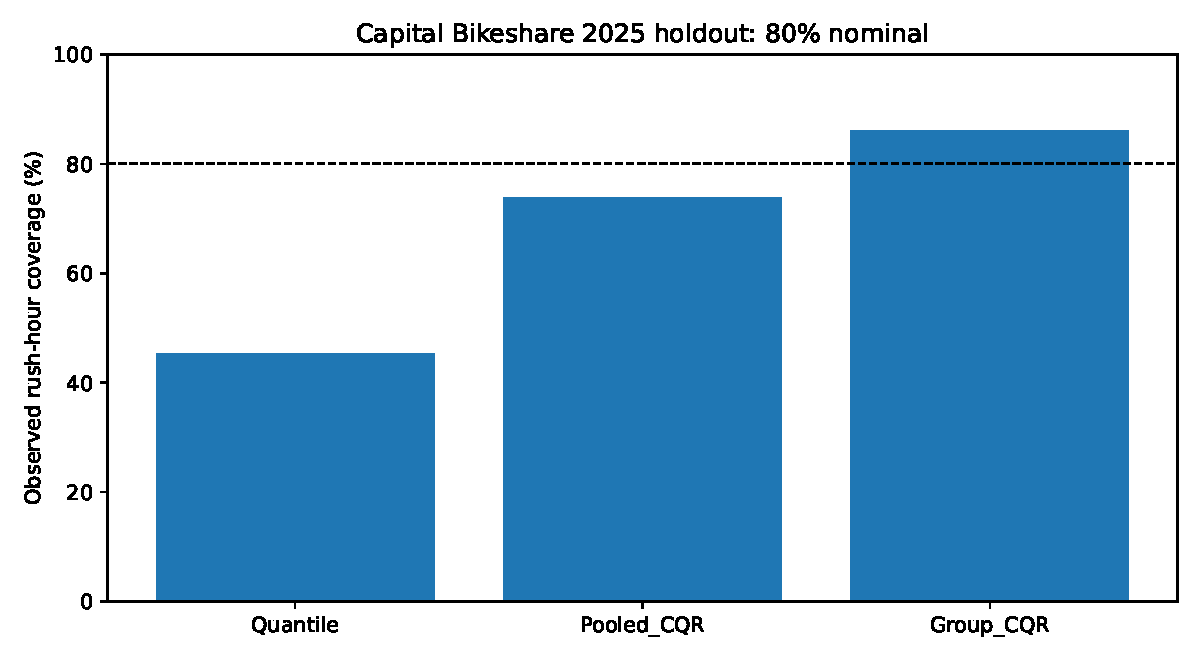
\includegraphics[width=.96\linewidth,draft=false]{modern_coverage.pdf}
\caption{Coverage and interval width from the modern 2025 evaluation, as supplied by the reproducible analysis pipeline.}\label{fig:modern}\end{figure}
Group-wise calibration improves rush-period empirical coverage by 12.29 percentage points, while the mean rush-period interval becomes 261.26 trip starts (22.7\%) wider. Overall coverage changes little. An independent 3,000-draw date-cluster bootstrap based on the submitted individual predictions gives a descriptive 95\% percentile interval of 10.7--14.0 percentage points for the rush-period difference; the separate run report gives 10.6--13.9 points. Differences are consistent with distinct bootstrap seeds. The metrics table was independently recomputed from 26,280 method-specific prediction rows (8,760 hourly outcomes evaluated under three methods). In a subsequent local source-file audit, the authors verified all 24 original ZIP SHA-256 hashes and reproduced every hourly count without discrepancies. This check establishes reproducibility of the reported wall-clock aggregation, not unique recovery of the repeated autumn daylight-saving hour.
\subsection{Historical benchmark as context}
\begin{table}[ht]\centering\caption{Historical UCI 2012 evaluation with forecast-time-available calendar predictors; not directly comparable in count scale with modern records.}\label{tab:historical}
\begin{tabular}{lrrr}\toprule
Method & Overall coverage (\%) & Rush coverage (\%) & Rush mean width\\\midrule
Quantile regression & 39.1 & 24.2 & 263.8\\
Pooled CQR & 80.5 & 56.3 & 466.6\\
Group CQR & 81.2 & 73.5 & 545.3\\\bottomrule\end{tabular}\end{table}
The independently rerun historical group-wise rush coverage gain is 17.1 percentage points (73.5\% versus 56.3\%), likewise associated with greater peak-hour width. We treat this as replication of a qualitative within-dataset comparison rather than an estimate of change between 2012 and 2025.

\subsection{Monthly instability within the contemporary evaluation}
We also evaluated coverage by calendar month within the fixed 2025 holdout, without updating or recalibrating either method. Figure~\ref{fig:monthly} displays the empirical rush-hour coverage for each month. This analysis is descriptive and was added as a temporal diagnostic; it is not an additional independent validation data set. Table~\ref{tab:monthly} gives the corresponding numbers. Group CQR exceeds pooled CQR during each of the twelve months, but the magnitude of improvement varies. For instance, in April the rush-hour coverage increases from 55.7\% to 66.7\%, whereas in August the respective values are 97.2\% and 99.1\%. The improvement is therefore not evidence of uniform attainment of nominal 80\% coverage over time; group CQR also falls below 80\% during several months. The seasonal variation reinforces the need to report time-local reliability in addition to a single annual average.
\begin{table}[ht]\centering
\caption{2025 monthly rush-hour empirical coverage (percent). The same models and calibration data were used throughout; values are descriptive.}\label{tab:monthly}
\begin{tabular}{lrrr}\toprule
Month & Rush hours & Pooled CQR & Group CQR \\\midrule
01 & 217 & 94.9 & 98.2 \\
02 & 196 & 79.1 & 88.8 \\
03 & 217 & 61.3 & 77.9 \\
04 & 210 & 55.7 & 66.7 \\
05 & 217 & 57.6 & 75.1 \\
06 & 210 & 72.9 & 85.7 \\
07 & 217 & 74.2 & 89.9 \\
08 & 217 & 97.2 & 99.1 \\
09 & 210 & 61.9 & 84.3 \\
10 & 217 & 80.6 & 94.5 \\
11 & 210 & 85.7 & 92.9 \\
12 & 217 & 65.0 & 80.6 \\
\bottomrule
\end{tabular}\end{table}
\begin{figure}[ht]\centering
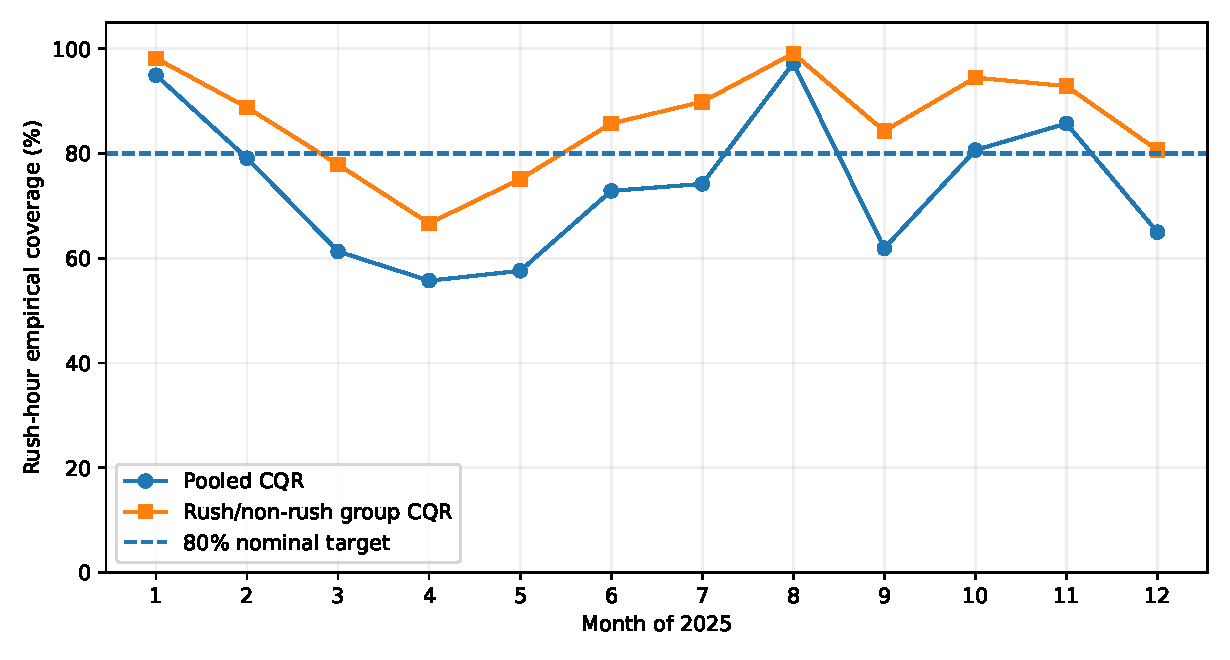
\includegraphics[width=.95\linewidth,draft=false]{monthly_peak_coverage.pdf}
\caption{Monthly rush-hour coverage in 2025 for pooled and group-calibrated conformal intervals. The dashed line indicates the nominal 80\% target, not a guaranteed conditional coverage level.}\label{fig:monthly}
\end{figure}

\subsection{Daylight-saving time sensitivity}
The hourly aggregation uses local wall-clock labels. On 9 March 2025, 02:00 is a nonexistent local hour yet the regular grid contains a zero-count row; on 2 November 2025, the repeated 01:00 period is represented by one label. We therefore removed both affected labels from the held-out 2025 predictions without retraining or recalibration. Table~\ref{tab:dst} reports the full and reduced-sample empirical coverage. Since both labels are non-rush periods, rush-hour metrics are identical by construction. This sensitivity check tests the influence of the affected rows on reported metrics; it does not validate source-level timestamp interpretation.
\begin{table}[ht]\centering\caption{Effect of excluding two 2025 daylight-saving clock labels (9 March 02:00; 2 November 01:00). Coverage in percent.}\label{tab:dst}\begin{tabular}{lrrr}\toprule Method & Full $n=8760$ & Reduced $n=8758$ & Rush full/reduced \\\midrule
Quantile & 52.05 & 52.07 & 45.28 \\
Pooled CQR & 86.24 & 86.25 & 73.86 \\
Group CQR & 85.98 & 85.99 & 86.14 \\
\bottomrule\end{tabular}\end{table}

\subsection{Upper-tail exceedances and a decision-oriented sensitivity analysis}
Coverage gives equal weight to misses above and below the interval. In contrast, planning against unexpectedly high trip-start demand focuses attention on the upper limit $U_t$. We therefore calculate the upper-exceedance frequency $\Pr_{\mathrm{emp}}(Y_t>U_t)$ and the mean positive exceedance $E_{\mathrm{emp}}[(Y_t-U_t)_+]$ in 2,555 prespecified peak-hour bins. These measures are diagnostics of \emph{recorded} departures; they are not direct counts of unmet trips.

To examine dependence on decision priorities without inventing financial costs, we construct a stylized planning-capacity proxy in which $U_t$ is interpreted as a hypothetical capacity target. As defined in Equation~\eqref{eq:loss}, the proxy weights positive exceedances by the user-chosen cost ratio $\lambda$.
The first term represents unused hypothetical capacity and the second penalizes demand above that level. Both are expressed in trip-start equivalents, not money or observed fleet costs. The parameter $\lambda$ is the assumed relative cost per unit of under-capacity. Since bike trips can be blocked by real supply constraints, observed trip starts are not unconstrained latent demand. Thus this is a descriptive sensitivity analysis, not a validated optimization or rebalancing policy.

\begin{table}[ht]\centering\small
\caption{Peak-hour 2025 diagnostics and hypothetical asymmetric-capacity loss, computed from the 2,555 paired hourly interval predictions. Percentages represent empirical frequencies; positive exceedance and loss values are in trip-start equivalents per hour.}\label{tab:policy}
\begin{tabular}{lrrrr}\toprule
Method & Upper miss (\%) & Positive exceedance & $\overline L_2$ & $\overline L_{10}$ \\\midrule
Quantile regression & 43.33 &108.24&448.98&1314.90\\
Pooled CQR &20.70&38.82&460.86&771.46\\
Groupwise CQR &11.19&17.35&533.45&672.29\\
\bottomrule\end{tabular}\end{table}

The groupwise procedure reduces the rate of upper misses from 20.70\% to 11.19\% and the mean positive exceedance from 38.82 to 17.35 trips/h compared with pooled CQR. The latter represents a 55.3\% reduction in positive exceedance on this test sample. Nevertheless, it also increases the mean positive unused margin from 383.21 to 498.74 trips/h. Thus groupwise intervals need not be preferable under every assumed cost ratio.

The two CQR choices have equal sample-average proxy loss at $\lambda^*=5.38$, obtained algebraically from the observed mean unused-margin and exceedance differences. Below this threshold, pooled CQR has smaller sample-average loss; above it, groupwise CQR has smaller sample-average loss. A descriptive paired day-resampling bootstrap gives an approximate 95\% percentile interval of 4.49--6.56 for the break-even ratio. The ratio is a feature of this particular data set, fixed split, and upper-bound decision proxy. It is not an empirically estimated transport-agency cost ratio. It must \emph{not} be interpreted as a proven optimum for fleet sizing, unmet-demand management or actual dispatch operations.

\section{Discussion}
\subsection{Why overall coverage alone is insufficient}
The overall empirical coverage of pooled CQR is above the nominal 80\% level in the contemporary evaluation, yet peak-hour coverage is substantially below target. This is not logically inconsistent: pooled coverage is an average across unequally sized subsets. The large non-rush subgroup, with higher observed coverage, can mask systematic shortfalls in the smaller peak subgroup. Consequently, a single annual metric is insufficient when decision-relevant operating conditions are known in advance.

\subsection{Coverage improvements are accompanied by width and decision-proxy costs}
Separate calibration raises peak-hour coverage without modifying the fitted quantile functions. It does so by increasing the calibration expansion for the peak subgroup; interval width therefore matters as much as the number of observations covered. In the 2025 holdout the gain of 12.29 percentage points coincides with 261.26 additional trip starts in mean peak-hour interval width. The decision-proxy sensitivity in Table~\ref{tab:policy} clarifies why a narrower pooled interval may be preferred under low hypothetical under-capacity penalties, whereas the groupwise interval may be preferred when shortfalls are heavily penalized. No actual fleet stockouts, agency costs, or counterfactual trips are observed, so the analysis does not identify an optimal real-world policy.

\subsection{Monthly robustness and temporal shift}
Annual peak coverage of 86.1\% under group CQR does not imply stable month-specific coverage. April remains below target at 66.7\%, while August reaches 99.1\%. The same held-out predictions and fixed calibration thresholds were used for every month. These diagnostics document nonuniform empirical reliability but do not isolate whether seasonal covariate shift, response drift, calendar-only model misspecification or changing service conditions account for the observed pattern.

\subsection{Implications for transport performance reporting and management}
The results suggest a concrete change in how shared-mobility forecast systems can be reported to planners: pair an annual coverage figure with at least one predeclared operational-time subgroup, a month-by-month reliability display, direction-specific miss rates and interval width. For this particular case, reporting only the 86.2\% annual coverage of pooled CQR would suppress a 12.3-percentage-point difference between it and groupwise peak-hour calibration. A reporting protocol that shows both intervals prevents operators from mistaking a nominal coverage label for an equivalent level of protection in all planning windows.

These findings do \emph{not} authorize choosing a rebalancing strategy from this dataset alone. Actual deployment would require station-level available inventory, bike availability before each hour, vehicle relocation lead times, capacity constraints, travel times and user-relevant service outcomes. At minimum, a prospective operations trial should specify the action generated by each interval, evaluate realized service losses and transport equity consequences, and assess forecast drift with rolling or refreshed calibration periods. This is a proposed evaluation framework, not a claim that any such intervention was conducted.

\subsection{Limitations and scope of generalization}
This paper considers one system, one fixed chronological partition and one calendar-only base modeling strategy. Neither finite-sample coverage under the actual temporal shift nor transport-system performance is guaranteed. Group labels are known before forecasting but are based on clock hours, not observed commuting purposes; weekends and holidays remain in their clock-defined categories. Trip starts represent fulfilled departures rather than unconstrained latent demand. Station-level shortages and rebalancing outcomes are not observed.

The asymmetric-capacity analysis is illustrative, with hypothetical loss weights and upper interval endpoints rather than optimized capacity decisions. It measures exposure against observed departures and cannot quantify unmet travel. The daylight-saving sensitivity test demonstrates that two identified clock labels have negligible influence on the reported aggregate coverage; it cannot validate the original hour reconstruction from the source trip timestamps. Likewise, comparing the UCI historical dataset with contemporary Capital Bikeshare records is a qualitative comparison of within-source coverage gaps, not an estimate of changes in the level of demand.

No adaptive conformal benchmark or alternative chronological retraining scheme was executed for this manuscript. Claims of general superiority over adaptive methods or deployment readiness are therefore outside its scope. The original monthly archives and calendar-hour aggregation have been verified against source hashes and counts, and the primary fitted-model outputs were exactly reproduced from the audited hourly series. A public versioned code-and-output deposit, independently rerunnable by external researchers, remains to be completed; the historical UCI secondary evaluation was not included in the primary-model re-execution.
\section{Conclusions}
This study evaluated whether aggregate predictive-interval reliability is informative about demand uncertainty at operationally recognizable times in a contemporary shared-bicycle system. Three established interval procedures were evaluated on a strictly later calendar year, allowing the comparison to describe realized out-of-time behavior rather than in-sample goodness of fit. The first result is a pronounced aggregation discrepancy: pooled CQR covers 86.2\% of all 2025 hours while covering only 73.9\% of predefined peak hours. In this setting, an annual coverage report alone gives an incomplete picture of the intervals available to planners.

Separate calibration for peak and non-peak hours improves observed peak-hour coverage to 86.1\%, a 12.29-percentage-point increase, while widening peak-hour intervals by 22.7\%. The results therefore support an explicit coverage--efficiency evaluation rather than a blanket claim that one calibrated method dominates another. Direction-specific assessment reveals a related asymmetry: upper-bound exceedance frequency decreases from 20.7\% to 11.2\%, and mean positive exceedance decreases by 55.3\%. These are exceedances of recorded departures relative to predictions, not direct evidence of fewer bicycle stockouts.

The decision-oriented sensitivity analysis adds an important qualification. If one uses interval upper endpoints as hypothetical capacity targets, the method preferred by a simple asymmetric loss changes with the analyst's assumed penalty on under-capacity. In this sample, the pooled and groupwise CQR loss curves intersect near $\lambda=5.38$. Because no operator cost coefficients, actual supply constraints or unmet trips were observed, this threshold should inform sensitivity thinking, not real-world dispatch prescriptions.

Two further observations temper the favorable annual assessment of groupwise CQR. Monthly peak-hour coverage fluctuates substantially, falling below the 80\% target in several months. And the older UCI benchmark reveals a comparable within-dataset coverage--width trade-off without permitting direct historical comparisons of trip-volume levels. Taken together, the empirical evidence motivates subgroup reporting, direction-sensitive interval diagnostics and transparent sensitivity checks when predictive uncertainty is used in transport planning.

The study's main limitation is also its boundary of contribution: it evaluates established procedures for one system, one fixed split and one calendar-only forecasting model; it does not offer new conformal theory, a deployed forecasting framework or a tested fleet rebalancing intervention. The most relevant future validation would combine verified timezone-aware reconstruction, additional metropolitan systems, realistic forecast features and observed operational constraints to test whether the diagnostic differences translate into better capacity or service decisions. Until such validation, the reported findings should be treated as reproducible sample-conditional evidence about prediction-interval reliability, not a claim of guaranteed future coverage or improved transportation outcomes.

\section*{Author Contributions}
Pedro Ramos De Santis led the conceptualization, research design, statistical methodology, computational implementation, formal analysis, interpretation of results, and writing of the original draft. Carlos Mart\'in Barreiro contributed to the study design, methodological review, interpretation of findings, and critical revision of the manuscript. Both authors reviewed the manuscript and share responsibility for approving the version submitted for publication.

\section*{Declaration of Conflicting Interests}
The authors declared no potential conflicts of interest with respect to the research, authorship, and/or publication of this article.

\section*{Funding}
The authors disclosed no financial support for the research, authorship, and/or publication of this article.

\section*{Data and Code Availability}
Capital Bikeshare monthly trip histories (2024--2025) are publicly available at \url{https://capitalbikeshare.com/system-data}; the historical UCI Bike Sharing dataset is accessible at \url{https://doi.org/10.24432/C5W894}. The 24 archived Capital Bikeshare source hashes matched the original inputs, and independent reaggregation recovered 12,775,227 trip starts and 17,544 local-clock hourly observations with no hourly-count discrepancies. The modern forecasting experiment reproduced all 26,280 prediction rows and nine summary metric rows exactly. The historical 2011--2012 benchmark was independently re-estimated using calendar-only predictors and the documented 2011 training, January--June 2012 calibration, and July--December 2012 evaluation split (4,376 test observations). A version-controlled reproduction package containing analysis code, required dependencies, derived data, predictions, diagnostic outputs, and execution instructions has been prepared for deposit. \emph{A permanent public repository or archival DOI has not yet been assigned and must be inserted before submission.} The 24 original Capital Bikeshare ZIP files are not redistributed. The local-clock source aggregation merges the repeated autumn daylight-saving hour and does not identify both UTC occurrences separately.

\section*{Generative AI Disclosure}
OpenAI's ChatGPT was used during development of this manuscript to assist with research planning, literature discovery, generation and review of Python/LaTeX code, preparation and interpretation of statistical summaries, and drafting and revision of manuscript text. This disclosure includes assistance that may affect the description of methods, results, and conclusions; it is not limited to grammar or spelling correction. ChatGPT was not designated as an author. The named authors retain full responsibility for independent verification of data processing, computations, references, factual statements, and the final manuscript, and must confirm such verification before submission. No AI-generated observations were used as replacements for the reported bike-sharing trip records.

\begin{thebibliography}{99}
\bibitem[Angelopoulos and Bates(2023)]{angelopoulos2023} Angelopoulos, A. N., Bates, S. (2023). Conformal Prediction: A Gentle Introduction. \emph{Foundations and Trends in Machine Learning} 16(4), 494--591. \url{https://doi.org/10.1561/2200000101}.
\bibitem[Barber et~al.(2023)]{barber2023} Barber, R. F., Cand\`es, E. J., Ramdas, A., Tibshirani, R. J. (2023). Conformal Prediction Beyond Exchangeability. \emph{Annals of Statistics} 51(2), 816--845. \url{https://doi.org/10.1214/23-AOS2276}.
\bibitem[Behroozi and Edrisi(2025)]{behroozi2025} Behroozi, A., Edrisi, A. (2025). Predicting travel demand of a bike sharing system using graph convolutional neural networks. \emph{Public Transport} 17, 281--317. \url{https://doi.org/10.1007/s12469-024-00371-w}.
\bibitem[Capital Bikeshare(2026)]{capitaldata} Capital Bikeshare. System Data, monthly trip-history archives. \url{https://capitalbikeshare.com/system-data}. Accessed October 2026.
\bibitem[Fanaee-T(2013)]{uci2013} Fanaee-T, H. (2013). Bike Sharing [Dataset]. UCI Machine Learning Repository. \url{https://doi.org/10.24432/C5W894}.
\bibitem[Fanaee-T and Gama(2013)]{fanaee2013} Fanaee-T, H., Gama, J. (2013). Event labeling combining ensemble detectors and background knowledge. \emph{Progress in Artificial Intelligence}. \url{https://doi.org/10.1007/s13748-013-0040-3}.
\bibitem[Gibbs and Cand\`es(2021)]{gibbs2021} Gibbs, I., Cand\`es, E. (2021). Adaptive Conformal Inference Under Distribution Shift. \emph{Advances in Neural Information Processing Systems} 34.
\bibitem[Koenker and Bassett(1978)]{koenker1978} Koenker, R., Bassett, G. Jr. (1978). Regression Quantiles. \emph{Econometrica} 46(1), 33--50. \url{https://doi.org/10.2307/1913643}.
\bibitem[Rennie et~al.(2023)]{rennie2023} Rennie, N., Cleophas, C., Sykulski, A. M., Dost, F. (2023). Analysing and visualising bike-sharing demand with outliers. \emph{Discover Data}. \url{https://doi.org/10.1007/s44248-023-00001-z}.
\bibitem[Romano et~al.(2019)]{romano2019} Romano, Y., Patterson, E., Cand\`es, E. J. (2019). Conformalized Quantile Regression. \emph{Advances in Neural Information Processing Systems} 32, 3543--3553.
\bibitem[Shafer and Vovk(2008)]{shafer2008} Shafer, G., Vovk, V. (2008). A Tutorial on Conformal Prediction. \emph{Journal of Machine Learning Research} 9, 371--421.
\bibitem[Vovk(2012)]{vovk2012} Vovk, V. (2012). Conditional validity of inductive conformal predictors. \emph{Proceedings of Machine Learning Research} 25, 475--490.
\bibitem[Yang et~al.(2026)]{yang2026} Yang, C., Huang, X., Qiu, S., Cheng, Y. (2026). CONTINA: Confidence interval for traffic demand prediction with coverage guarantee. \emph{Transportation Research Part C}, 184, 105502. \url{https://doi.org/10.1016/j.trc.2025.105502}.
\bibitem[Yang et~al.(2020)]{yangspace2020} Yang, L., Zhang, F., Kwan, M.-P., Wang, K., Zuo, Z., Xia, S., Zhang, Z., Zhao, X. (2020). Space-time demand cube for spatial-temporal coverage optimization model of shared bicycle system: A study using big bike GPS data. \emph{Journal of Transport Geography} 88, 102861. \url{https://doi.org/10.1016/j.jtrangeo.2020.102861}.
\end{thebibliography}
\end{document}
